\section{Testplan}

Der Testplan beschreibt alle wichtigen Testfälle und ihre erwarteten Resultate.

\subsection{Ablaufplan}
\begin{figure}[h!]
	\centering
	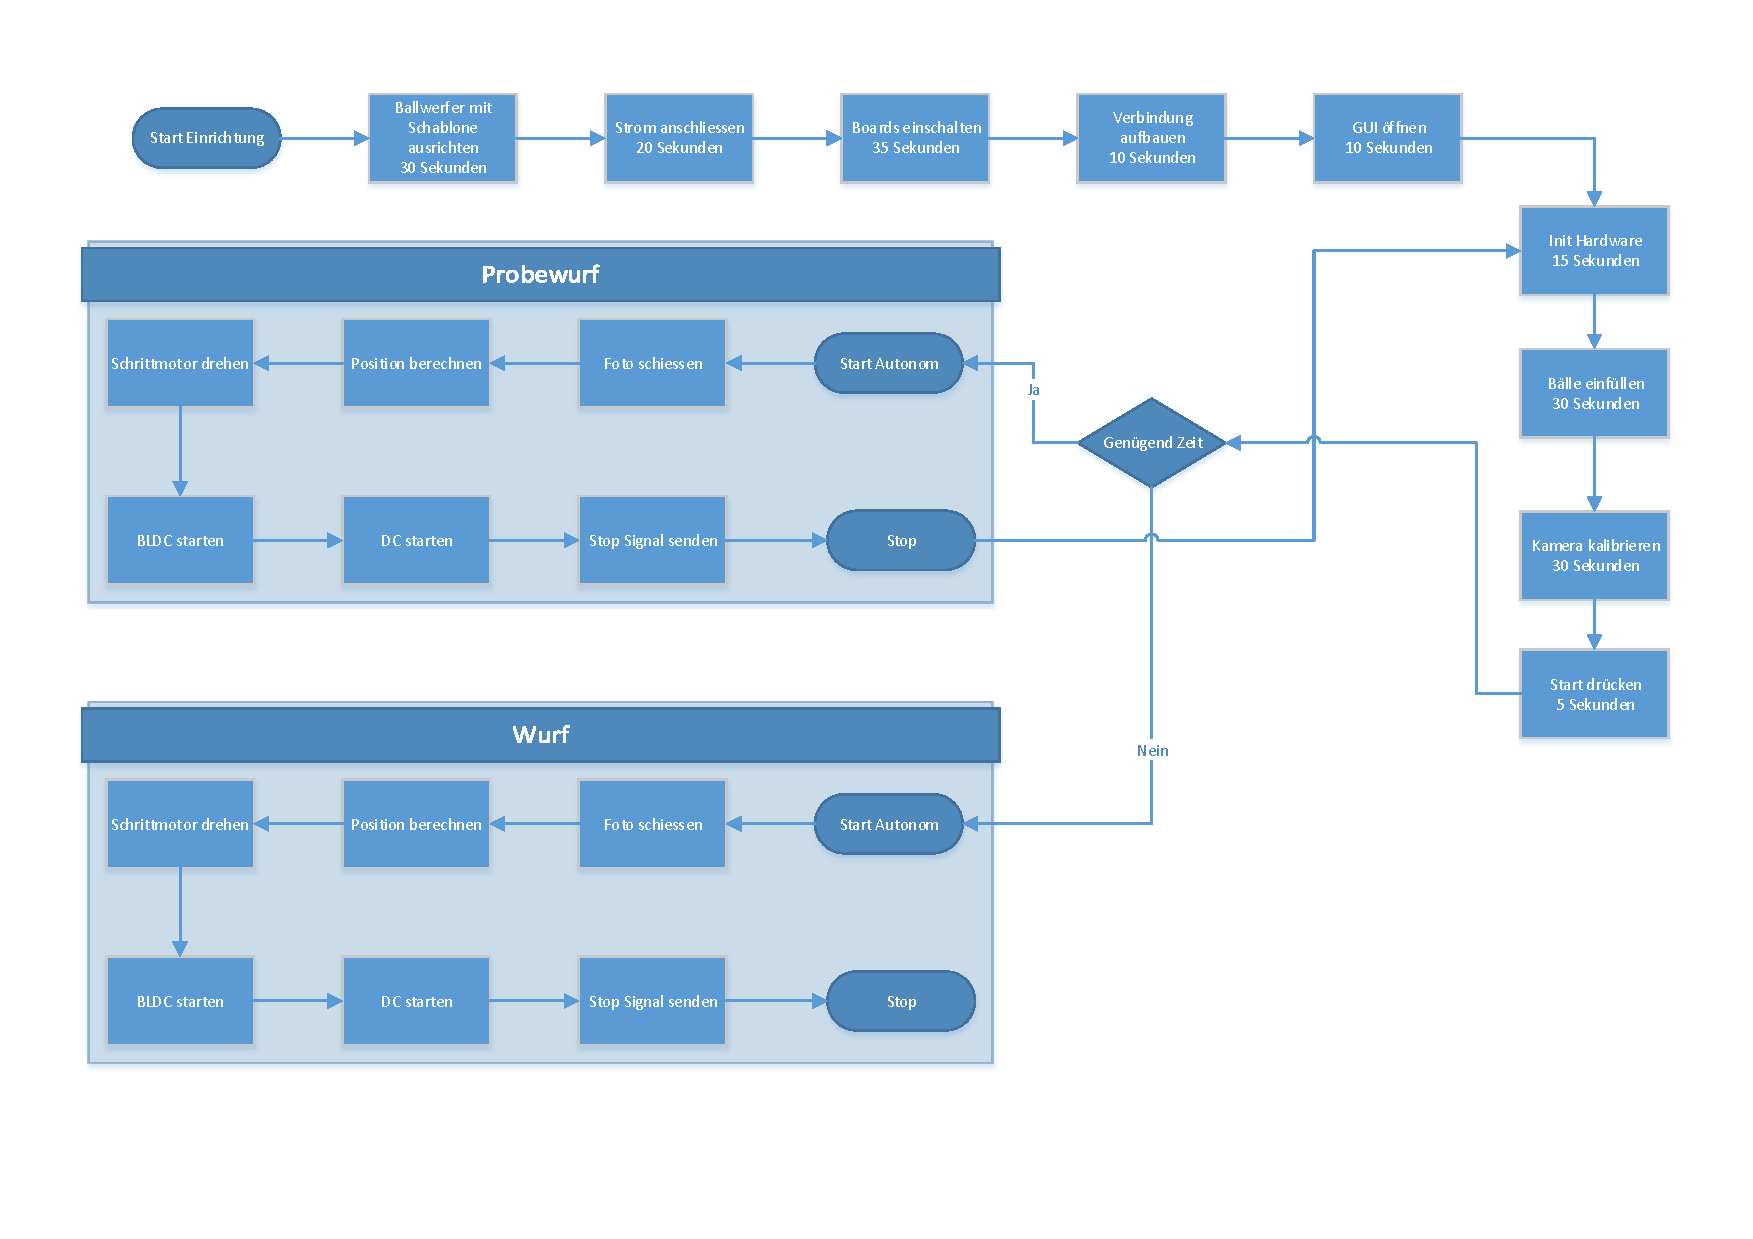
\includegraphics[width=0.7\linewidth]{../../fig/ablauf-ballwurf}
	\caption{}
	\label{fig:ablauf-ballwurf}
\end{figure}


\subsection{Gesamtsystemtest}

Im Gesamtsystemtest wird der Ballwerfer als Ganzes getestet. Im speziellen wird der Ablauf bei einem Probewurf simuliert.

\subsubsection{Reihenfolge der Testdurchführung}
GST101, GST102, GST103, GST104, GST105, GST106, GST107, GST108

\subsubsection{GST101 Ballwerfer ausgerichtet}
\begin{table}[h!]
	\renewcommand{\arraystretch}{1.5}
	\begin{tabular}{|r|p{14cm}|}
		\hline Beschreibung & Ballwerfer ist mit der Schablone auf dem Spielfeld mittig ausgerichtet. \\ 
		\hline Vorbedingungen &  \\ 
		\hline Testdaten & Konfigurationsdaten \\ 
		\hline Vorgehen & 
		\begin{enumerate}
			\item Schablone auflegen
			\item Ballwerfer auf die Mitte stellen
			\item Schablone entfernen
		\end{enumerate} \\ 
		\hline Ergebnis & Der Ballwerfer steht in der Mitte des Spielfeld.s \\ 
		\hline 
	\end{tabular}
\end{table}

\subsubsection{GST102 Strom angeschlossen}
\begin{table}[h!]
	\renewcommand{\arraystretch}{1.5}
	\begin{tabular}{|r|p{14cm}|}
		\hline Beschreibung & Alle Komponenten sind am Strom angeschlossen. \\ 
		\hline Vorbedingungen &  GST101\\ 
		\hline Testdaten & Konfigurationsdaten \\ 
		\hline Vorgehen & 
		\begin{enumerate}
			\item Netzteil am Strom anschliessen
			\item Rasperry am Netzteil anschliessen
			\item Freedom Board am Netzteil anschliessen
			\item DC Motor am Netzteil anschliessen
			\item BLDC Motor am Netzteil anschliessen
			\item STP Motor am Netzteil anschliessen
		\end{enumerate} \\ 
		\hline Ergebnis & Alle Komponenten sind am Strom angeschlossen und lassen sich in Betrieb nehmen. \\ 
		\hline 
	\end{tabular}
\end{table}
\newpage

\subsubsection{GST103 Boards eingeschaltet}
\begin{table}[h!]
	\renewcommand{\arraystretch}{1.5}
	\begin{tabular}{|r|p{14cm}|}
		\hline Beschreibung & Freedom Board und Rasperry einschalten. \\ 
		\hline Vorbedingungen &  GST102\\ 
		\hline Testdaten & Konfigurationsdaten \\ 
		\hline Vorgehen & 
		\begin{enumerate}
			\item Freedom Board einschalten
			\item Rasperry einschalten
		\end{enumerate} \\ 
		\hline Ergebnis & Freedom Board und Rasperry sind in Betrieb. \\ 
		\hline 
	\end{tabular}
\end{table}

\subsubsection{GST104 Verbindung aufgebaut}
\begin{table}[h!]
	\renewcommand{\arraystretch}{1.5}
	\begin{tabular}{|r|p{14cm}|}
		\hline Beschreibung & Computer ist mit dem Rasperry WLAN verbunden. \\ 
		\hline Vorbedingungen &  GST103\\ 
		\hline Testdaten & Konfigurationsdaten \\ 
		\hline Vorgehen & 
		\begin{enumerate}
			\item Computer einschalten
			\item WLAN verbinden
			\item WLAN Login
		\end{enumerate} \\ 
		\hline Ergebnis & Computer ist mit dem Rasperry WLAN verbunden. \\ 
		\hline 
	\end{tabular}
\end{table}

\subsubsection{GST105 GUI geöffnet}
\begin{table}[h!]
	\renewcommand{\arraystretch}{1.5}
	\begin{tabular}{|r|p{14cm}|}
		\hline Beschreibung & Der Configurator lässt sich auf dem Computer öffnen. \\ 
		\hline Vorbedingungen &  GST104\\ 
		\hline Testdaten & Konfigurationsdaten \\ 
		\hline Vorgehen & 
		\begin{enumerate}
			\item Configurator starten
		\end{enumerate} \\ 
		\hline Ergebnis & Der Configurator ist geöffnet und lässt sich bedienen. \\ 
		\hline 
	\end{tabular}
\end{table}
\newpage

\subsubsection{GST106 Reset Motoren}
\begin{table}[h!]
	\renewcommand{\arraystretch}{1.5}
	\begin{tabular}{|r|p{14cm}|}
		\hline Beschreibung & Alle Motoren haben einen Reset durchgeführt. \\ 
		\hline Vorbedingungen &  GST105\\ 
		\hline Testdaten & Konfigurationsdaten \\ 
		\hline Vorgehen & 
		\begin{enumerate}
			\item GUI Tab wechseln
			\item STP Motor reseten
			\item DC Motor reseten
			\item BLDC Motor reseten
		\end{enumerate} \\ 
		\hline Ergebnis & Alle Motoren haben ihren Ausgangsstatus. \\ 
		\hline 
	\end{tabular}
\end{table}

\subsubsection{GST107 Bälle eingefüllt}
\begin{table}[h!]
	\renewcommand{\arraystretch}{1.5}
	\begin{tabular}{|r|p{14cm}|}
		\hline Beschreibung & Die Bälle zum Abschuss einfüllen. \\ 
		\hline Vorbedingungen &  GST106\\ 
		\hline Testdaten & Konfigurationsdaten \\ 
		\hline Vorgehen & 
		\begin{enumerate}
			\item 5 Bälle einfüllen
		\end{enumerate} \\ 
		\hline Ergebnis & Der Ballwerfer ist geladen. \\ 
		\hline 
	\end{tabular}
\end{table}

\subsubsection{GST108 Kamera kalibriert}
\begin{table}[h!]
	\renewcommand{\arraystretch}{1.5}
	\begin{tabular}{|r|p{14cm}|}
		\hline Beschreibung & Kamera kalibrieren \\ 
		\hline Vorbedingungen &  GST104\\ 
		\hline Testdaten & Konfigurationsdaten \\ 
		\hline Vorgehen & 
		\begin{enumerate}
			\item GUI Tab wechseln
			\item Werte im Configurator einstellen
		\end{enumerate} \\ 
		\hline Ergebnis & Die Kamera ist so eingestellt, dass sie den Korb erkennt. \\ 
		\hline 
	\end{tabular}
\end{table}

\newpage
\subsection{Testplan-Maschinenbau}
\subsubsection{Funktionskontrolle Schrittmotor}
\begin{table}[h!]
	\renewcommand{\arraystretch}{1.5}
	\begin{tabular}{|r|p{14cm}|}
		\hline Beschreibung & Schrittmotor muss den Aufbau in beide Drehrichtungen über den Schwenkbereich drehen können  \\ 
		\hline Vorbedingungen & Aufbau montiert \\ 
		\hline Vorgehen & 
		\begin{enumerate}
			\item Schrittmotor nach links drehen lassen 
			\item Schrittmotor nach rechts drehen lassen
		\end{enumerate} \\ 
		\hline Ergebnis & Funktion IO/ NIO \\ 
		\hline Verbesserungen & Reibung verringern, Lagerung anpassen, Positionierung Schrittmotor anpassen \\ 
		\hline 
	\end{tabular}
\end{table}
\newpage

\subsubsection{Funktionskontrolle DC- Motor}
\begin{table}[h!]
	\renewcommand{\arraystretch}{1.5}
	\begin{tabular}{|r|p{14cm}|}
		\hline Beschreibung & DC-Motor muss die Bälle dem Drehrad zuführen können.  \\ 
		\hline Vorbedingungen & Aufbau montiert \\ 
		\hline Vorgehen & 
		\begin{enumerate}
			\item Motor in beide Drehrichtungen drehen lassen (ohne Bälle). 
			\item Test mit Bällen wiederholen
		\end{enumerate} \\ 
		\hline Ergebnis & Funktion IO/ NIO \\ 
		\hline Verbesserungen & Konstruktive Anpassungen, Drezahl des Motors anpassen \\ 
		\hline 
	\end{tabular}
\end{table}

\subsubsection{Funktionskontrolle BLDC- Motor}
\begin{table}[h!]
	\renewcommand{\arraystretch}{1.5}
	\begin{tabular}{|r|p{14cm}|}
		\hline Beschreibung & BLDC-Motor muss die Bälle auf die gewünschte Abwurfgeschwindigkeit beschleunigen.  \\ 
		\hline Vorbedingungen & Aufbau montiert \\ 
		\hline Vorgehen & 
		\begin{enumerate}
			\item BLDC- Motor auf gewünschter Drezahl Drehen lassen 
			\item Mechanischer Aufbau überprüfen
			\item Test mit Bällen wiederholen 
		\end{enumerate} \\ 
		\hline Ergebnis & Funktion IO/ NIO \\ 
		\hline Verbesserungen & Konstruktive Anpassungen, Drezahl des Motors anpassen, Gegendruckplatte konstruktiv anpassen \\ 
		\hline 
	\end{tabular}
\end{table}
\newpage

\subsubsection{Stabilität Aufbau}
\begin{table}[h!]
	\renewcommand{\arraystretch}{1.5}
	\begin{tabular}{|r|p{14cm}|}
		\hline Beschreibung & Der Aufbau muss bei maximaler Drezahl aller Motoren stabil betrieben werden können. \\ 
		\hline Vorbedingungen & Funktionskontrolle der einzelnen Motoren gewährleistet. \\ 
		\hline Vorgehen & 
		\begin{enumerate}
			\item BLDC- Motor auf maximale Drezahl bringen
			\item 2 min drehen lassen 
			\item Schrittmotor mit max. Geschwindigkeit über den ganzen Schwenkbereich drehen lassen  
			\item DC- Motor einschalten
			\item Kontrolle des mechanischen Aufbaus
		\end{enumerate} \\ 
		\hline Ergebnis & Keine Schäden am Aufbau erkennbar/ Schäden am Aufbau erkennbar \\ 
		\hline Verbesserungen & Stabilität anpassen, Drehzahlbereich der Motoren einschränken \\ 
		\hline 
	\end{tabular}
\end{table}

\subsubsection{Funktionskontrolle Treffgenauigkeit }
\begin{table}[h!]
	\renewcommand{\arraystretch}{1.5}
	\begin{tabular}{|r|p{14cm}|}
		\hline Beschreibung & Die Bälle müssen in der gewünschten Zeit die gewünschte Treffgenauigkeit erreichen   \\ 
		\hline Vorbedingungen & Einzelfunktionskontrollen aller Motoren erfolgreich, Stabilität des Aufbaus erreicht \\ 
		\hline Vorgehen & 
		\begin{enumerate}
			\item BLDC- Motor auf gewünschter Drehzahl Drehen lassen 
			\item Ballnachschub starten 
		\end{enumerate} \\ 
		\hline Ergebnis & Funktion IO/ NIO \\ 
		\hline Verbesserungen & Konstruktive Anpassungen, Drezahl des Motors anpassen, Gegendruckplatte konstruktiv anpassen \\ 
		\hline 
	\end{tabular}
\end{table}

\clearpage
\subsection{Testplan-Elektrotechnik}
\subsection{Testplan-Elektrotechnik}
\subsubsection{KOM101 Kommunikation mit PC}
\begin{table}[h!]
	\renewcommand{\arraystretch}{1.5}
	\begin{tabular}{|r|p{13cm}|}
		\hline Beschreibung	&
			Das Freedomboard kann per USB/UART-Verbindung bedient werden. \\ 
		\hline Vorbedingungen	&
			Toolchain, Terminalprogramm und Python installiert \\ 
		\hline Testdaten	& - \\ 
		\hline Vorgehen		& 
		\begin{enumerate}
			\item Freedomboard verbinden
			\item Verbindung aufbauen mit Freedomboard
			\item Terminalverbindung eröffnen
			\item Reset des Freedomboards durchführen per Reset-Schalter
			\item Ausgabe begutachten und auf Bereitschaft warten
			\item Terminalverbindung schliessen
			\item Testskript durchführen
			\item Freedomboard trennen von PC 
		\end{enumerate} \\ 
		\hline Ergebnis 	&
			Das Freedomboard zeigt auf der Terminalverbindung nach dem
			Reset die Befehlsliste an. Das Testskript beendet erfolgreich.\\ 
		\hline 
	\end{tabular}
\end{table}

\newpage
\subsubsection{KOM102 Kommunikation mit RaspberryPi}
\begin{table}[h!]
	\renewcommand{\arraystretch}{1.5}
	\begin{tabular}{|r|p{13cm}|}
		\hline Beschreibung	&
			Das Freedomboard kann per USB/UART-Verbindung bedient werden. \\ 
		\hline Vorbedingungen	& Python installiert \\ 
		\hline Testdaten	& - \\ 
		\hline Vorgehen		& 
		\begin{enumerate}
			\item Freedomboard verbinden per USB Kabel
			\item Testskript durchführen
			\item Freedomboard trennen
		\end{enumerate} \\ 
		\hline Ergebnis 	&
			Das Testskript beendet erfolgreich.\\ 
		\hline 
	\end{tabular}
\end{table}

\newpage
\subsubsection{MOT101 Ballabwurf mit BLDC Motor}
\begin{table}[h!]
	\renewcommand{\arraystretch}{1.5}
	\begin{tabular}{|r|p{13cm}|}
		\hline Beschreibung	& Der BLDC Motor lässt sich via USB/UART ansteuern. \\ 
		\hline Vorbedingungen	& Shell ist auf dem Freedomboard implementiert. \\ 
		\hline Testdaten	& - \\ 
		\hline Vorgehen		& 
		\begin{enumerate}
			\item Freedomboard verbinden
			\item Verbindung aufbauen mit Freedomboard
			\item Motorspeisung einschalten
			\item Motor einschalten
			\item Geschwindigkeit einstellen in 10\% Schritten
			\item Geschwindigkeit auf 0 stellen
			\item Motor ausschalten
			\item Motorspeisung ausschalten 
		\end{enumerate} \\ 
		\hline Ergebnis 	&
			Der Motor verändert die Geschwindigkeit entsprechend
			den Einstellungen.\\ 
		\hline 
	\end{tabular}
\end{table}

\newpage
\subsubsection{MOT102 Ballnachschub mit DC Motor}
\begin{table}[h!]
	\renewcommand{\arraystretch}{1.5}
	\begin{tabular}{|r|p{13cm}|}
		\hline Beschreibung	& Der DC Motor lässt sich via USB/UART ansteuern. \\ 
		\hline Vorbedingungen	&
			Shell ist auf dem Freedomboard implementiert.
			DC-Treiberstufe implementiert. Positionsschalter implementiert. \\ 
		\hline Testdaten	& - \\ 
		\hline Vorgehen		& 
		\begin{enumerate}
			\item Freedomboard verbinden
			\item Verbindung aufbauen mit Freedomboard
			\item Motor in Mitte der Wegstrecke platzieren 
			\item Verbindungsaufbau PC-Freedomboard
			\item Motorspeisung einschalten
			\item Bewegungsrichtung auf aufwärts einstellen
			\item Motor einschalten
			\item Motor einige Zentimeter fahren lassen
			\item Motor ausschalten
			\item Bewegungsrichtung umstellen auf abwärts
			\item Motor einschalten
			\item Motor einige Zentimeter fahren lassen
			\item Motor ausschalten
			\item Bewegungsrichtung umstellen auf aufwärts
			\item Motor einschalten
			\item Warten bis Endschalter auslöst
			\item (Bewegungsrichtung umstellen)
			\item Motor einschalten
			\item Warten bis Endschalter auslöst
			\item Motorspeisung ausschalten
			\item Freedomboard trennen
		\end{enumerate} \\ 
		\hline Ergebnis 	&
			Der Motor bewegt sich entsprechend der eingestellten
			Bewegungsrichtung und lässt sich ein- und ausschalten.
			Die Endschalter stoppen die Bewegung des Motors. \\ 
		\hline 
	\end{tabular}
\end{table}

\newpage
\subsubsection{MOT103 Turmausrichtung mit Schrittmotor}
\begin{table}[h!]
	\renewcommand{\arraystretch}{1.5}
	\begin{tabular}{|r|p{13cm}|}
		\hline Beschreibung	&
			Schrittmotor kann per Freedomboard bedient werden. \\ 
		\hline Vorbedingungen	&
			Shell ist auf dem Freedomboard implementiert.
			Positionsschalter implementiert. \\ 
		\hline Testdaten	& - \\ 
		\hline Vorgehen		& 
		\begin{enumerate}
			\item Freedomboard verbinden
			\item Verbindung aufbauen zum Freedomboard
			\item Positionserkennung triggern
			\item LED auf Freedomboard beachten
			\item Positionstriggerung quittieren
			\item Motorspeisung einschalten
			\item Motor in verschiedenen Schrittweiten und Richtungen bewegen
			\item Motor ausschalten
			\item Freedomboard trennen
		\end{enumerate} \\ 
		\hline Ergebnis 	&
			Die LED auf dem Freedomboard reagiert auf die
			Positionstriggerung und kann per Shell quittiert werden.
			Der Motor reagiert entsprechend auf die Ansteuerung. \\ 
		\hline 
	\end{tabular}
\end{table}

\newpage
\subsubsection{POW101 Leistungsspeisung per Server-Netzteil}
\begin{table}[h!]
	\renewcommand{\arraystretch}{1.5}
	\begin{tabular}{|r|p{13cm}|}
		\hline Beschreibung	&
			Die 12 Volt Speisung kann per Servernetzteil versorgt werden. \\ 
		\hline Vorbedingungen	&
			Maschine ist komplettiert und alle Leistungskomponenten
			sind einsatzbereit. \\ 
		\hline Testdaten	& - \\ 
		\hline Vorgehen		& 
		\begin{enumerate}
			\item Freedomboard verbinden
			\item Verbindung aufbauen zum Freedomboard
			\item Motorspeisung einschalten
			\item DC Motor herunterfahren zum unteren Endschalter
			\item 5 Tennisbälle einführen
			\item Turm ausrichten an linken Anschlag
			\item BLDC Motor starten auf 75\% der Maximaldrehzahl
			\item DC Motor einschalten und auf oberen Anschlag fahren lassen
			\item Turm ausrichten an rechten Anschlag
			\item BLDC ausschalten
			\item Freedomboard trennen
		\end{enumerate} \\ 
		\hline Ergebnis 	&
			Die Nennspannung von 12 Volt weicht während dem gesamten
			Prozess um maximal $\pm10$\% ab. \\ 
		\hline 
	\end{tabular}
\end{table}

\newpage
\subsubsection{SEN101 Positionsschalter}
\begin{table}[h!]
	\renewcommand{\arraystretch}{1.5}
	\begin{tabular}{|r|p{13cm}|}
		\hline Beschreibung	&
			Software kann auf erreichen von Fixpositionen reagieren. \\ 
		\hline Vorbedingungen	&
			Shell ist auf dem Freedomboard implementiert.
			Positionsschalter implementiert. \\ 
		\hline Testdaten	& - \\ 
		\hline Vorgehen		& 
		\begin{enumerate}
			\item Freedomboard verbinden
			\item Verbindung aufbauen zum Freedomboard
			\item Positionserkennung triggern
			\item LED auf Freedomboard beachten
			\item Positionstriggerung quittieren
			\item Freedomboard trennen
		\end{enumerate} \\ 
		\hline Ergebnis 	&
			Die LED auf dem Freedomboard reagiert auf die
			Positionstriggerung und kann per Shell quittiert werden.\\ 
		\hline 
	\end{tabular}
\end{table}



\newpage
\subsection{Testplan-Informatik}

Es wird zwischen Integrations- (INT) und Systemtest (SYS) unterschieden. Ein Integrationstest
ist technisch getrieben und prüft das Zusammenspiel der Komponenten. Aus diesem
Grund wird empfohlen, dass solche Tests von den Entwicklern selber durchgeführt werden.
Systemtest hingegen sind benutzerorientiert. Diese testen das System als Ganzes.
Die Tests sind voneinander abhängig, darum ist die Reihenfolge der Testausführung
definiert. Denn ein Test kann als Vorbedingung für einen anderen Test gelten. 

In den Tests wird von Controller und Configurator gesprochen. Der Controller ist
das Raspberry Pi und der Configurator die externe Steuerungseinheit.
Die Motoren sind als BLDC, DC und STP abgekürzt.
BLDC ist der Motor für das Schwungrad, DC für den Ballvorschub und STP zum Drehen der Plattform.

\subsubsection{Reihenfolge der Testdurchführung}
INT101, INT102, INT103, INT104
SYS101, SYS102, SYS103, SYS104, SYS105, SYS106, SYS107




\subsubsection{INT101 Webservice Erreichbarkeit}
\begin{table}[h!]
	\renewcommand{\arraystretch}{1.5}
	\begin{tabular}{|r|p{14cm}|}
		\hline Beschreibung & Die Webservices auf dem Controller müssen erreichbar sein. \\ 
		\hline Vorbedingungen & Controller Setup \\ 
		\hline Testdaten & URL: http://IP-ADDRESS-CONTROLLER:PORT-CONTROLLER \\ 
		\hline Vorgehen & 
		\begin{enumerate}
			\item Browser öffnen und URL eingeben.
		\end{enumerate} \\ 
		\hline Ergebnis & Der Browser zeigt eine Willkommensseite an \\ 
		\hline 
	\end{tabular}
\end{table}

\subsubsection{INT102 Webservice Bild laden}
\begin{table}[h!]
	\renewcommand{\arraystretch}{1.5}
	\begin{tabular}{|r|p{14cm}|}
		\hline Beschreibung & Der Bild-Lade Webservice muss ein Bild zurückliefern. \\ 
		\hline Vorbedingungen & INT101 \\ 
		\hline Testdaten & URL: http://IP-ADDRESS-CONTROLLER:PORT-CONTROLLER/image \\ 
		\hline Vorgehen & 
		\begin{enumerate}
			\item Browser öffnen und URL eingeben
		\end{enumerate} \\ 
		\hline Ergebnis & Ein Bild wird angezeigt. \\ 
		\hline 
	\end{tabular}
\end{table}
\newpage

\subsubsection{INT103 Webservice Kamera Konfig laden}
\begin{table}[h!]
	\renewcommand{\arraystretch}{1.5}
	\begin{tabular}{|r|p{14cm}|}
		\hline Beschreibung & Der Kamera-Konfig-Lade Webservice muss ein JSON-File mit den aktuellen Einstellungen liefern. \\ 
		\hline Vorbedingungen & INT102 \\ 
		\hline Testdaten & URL: http://IP-ADDRESS-CONTROLLER:PORT-CONTROLLER/camera \\ 
		\hline Vorgehen & 
		\begin{enumerate}
			\item Browser öffnen und URL eingeben
		\end{enumerate} \\ 
		\hline Ergebnis & JSON-File mit aktuellen Einstellungen ist ersichtlich. \\ 
		\hline 
	\end{tabular}
\end{table}

\subsubsection{INT104 Webservice Kamera Konfig speichern}
\begin{table}[h!]
	\renewcommand{\arraystretch}{1.5}
	\begin{tabular}{|r|p{14cm}|}
		\hline Beschreibung & Der Kamera-Konfig-Speicher Webservice muss ein JSON-File entgegennehmen und die Einstellungen speichern. \\ 
		\hline Vorbedingungen & INT103 \\ 
		\hline Testdaten & URL: http://IP-ADDRESS-CONTROLLER:PORT-CONTROLLER/camera \\ 
		\hline Vorgehen & 
		\begin{enumerate}
			\item Aktuelle Controller Einstellungen laden.
			\item Einstellungen in ein JSON-File speichern.
			\item Ein paar Werte anpassen.
			\item PUT Request an die URL senden mit dem JSON-File.
			\item Controller neu starten
			\item Aktuelle Controller Einstellungen laden.
		\end{enumerate} \\ 
		\hline Ergebnis & Die Einstellungen müssen nun die gleichen sein wie vor dem Neustart. \\ 
		\hline 
	\end{tabular}
\end{table}
\newpage

\subsubsection{SYS101 Configurator startet}
\begin{table}[h!]
	\renewcommand{\arraystretch}{1.5}
	\begin{tabular}{|r|p{14cm}|}
		\hline Beschreibung & Der Configurator lässt sich starten. \\ 
		\hline Vorbedingungen & Configurator Setup \\ 
		\hline Testdaten &  \\ 
		\hline Vorgehen & 
		\begin{enumerate}
			\item Configurator starten
		\end{enumerate} \\ 
		\hline Ergebnis & Es erscheint eine Benutzeroberfläche. \\ 
		\hline 
	\end{tabular}
\end{table}

\subsubsection{SYS102 Configurator Verbindungseinstellungen }
\begin{table}[h!]
	\renewcommand{\arraystretch}{1.5}
	\begin{tabular}{|r|p{14cm}|}
		\hline Beschreibung & Im Configurator lassen sich die Verbindungseinstellungen zum Controller ändern. \\ 
		\hline Vorbedingungen & SYS101 \\ 
		\hline Testdaten & Eigene Verbindungsdaten definieren \\ 
		\hline Vorgehen & 
		\begin{enumerate}
			\item Configurator starten
			\item Verbindungeinstellungen ändern und speichern
			\item Configurator neu starten
		\end{enumerate} \\ 
		\hline Ergebnis & Verbindungseinstellungen sind auch nach dem Neustart erhalten. \\ 
		\hline 
	\end{tabular}
\end{table}

\subsubsection{SYS103 Configurator Bild laden }
\begin{table}[h!]
	\renewcommand{\arraystretch}{1.5}
	\begin{tabular}{|r|p{14cm}|}
		\hline Beschreibung & Aktuelle Foto lässt sich laden und im Configurator anzeigen. \\ 
		\hline Vorbedingungen & SYS102 \\ 
		\hline Testdaten & Verbindungsdaten definieren, Bild \\ 
		\hline Vorgehen & 
		\begin{enumerate}
			\item Configurator starten
			\item Bild laden
		\end{enumerate} \\ 
		\hline Ergebnis & Aktuelles Foto erscheint im GUI. Auf dem Bild muss der Korb markiert sein und der Winkel angegeben. \\ 
		\hline 
	\end{tabular}
\end{table}
\newpage

\subsubsection{SYS104 Configurator Bild Konfiguration anwenden }
\begin{table}[h!]
	\renewcommand{\arraystretch}{1.5}
	\begin{tabular}{|r|p{14cm}|}
		\hline Beschreibung & Die Kamera-Einstellungen lassen sich editieren und auf den Controller anwenden. \\ 
		\hline Vorbedingungen & SYS103 \\ 
		\hline Testdaten & Konfigurationsdaten \\ 
		\hline Vorgehen & 
		\begin{enumerate}
			\item Configurator starten
			\item Kamera-Einstellunge editieren
			\item Kamera-Einstellung speichern
			\item Bild neu laden
		\end{enumerate} \\ 
		\hline Ergebnis & Auf dem GUI erscheint die Meldung, dass die Konfiguration erfolgreich gespeichert wurde.
		Ausserdem erscheint das Bild, welches mit den aktuellen Einstellungen modifiziert wurden. \\ 
		\hline 
	\end{tabular}
\end{table}

\subsubsection{SYS105 BLDC ansteuern}
\begin{table}[h!]
	\renewcommand{\arraystretch}{1.5}
	\begin{tabular}{|r|p{14cm}|}
		\hline Beschreibung & Der BLDC Motor lässt sich via GUI ansteuern. \\ 
		\hline Vorbedingungen & SYS102 \\ 
		\hline Testdaten & Konfigurationsdaten \\ 
		\hline Vorgehen & 
		\begin{enumerate}
			\item Configurator starten
			\item RPM anpassen
			\item Motor starten
			\item Motor stoppen
			\item Motor reset
		\end{enumerate} \\ 
		\hline Ergebnis & Der Motor wird sich in der entsprechenden Geschwindigkeit drehen. \\ 
		\hline 
	\end{tabular}
\end{table}
\newpage

\subsubsection{SYS106 DC ansteuern }
\begin{table}[h!]
	\renewcommand{\arraystretch}{1.5}
	\begin{tabular}{|r|p{14cm}|}
		\hline Beschreibung & Der DC Motor lässt sich via GUI ansteuern. \\ 
		\hline Vorbedingungen & SYS102 \\ 
		\hline Testdaten & Konfigurationsdaten \\ 
		\hline Vorgehen & 
		\begin{enumerate}
			\item Configurator starten
			\item Motor starten
			\item Motor stoppen
			\item Motor reset
		\end{enumerate} \\ 
		\hline Ergebnis & Der Motor wird sich drehen. Zusätzlich nimmt er seine Ausgangsposition beim Reset an.\\ 
		\hline 
	\end{tabular}
\end{table}

\subsubsection{SYS107 STP ansteuern}
\begin{table}[h!]
	\renewcommand{\arraystretch}{1.5}
	\begin{tabular}{|r|p{14cm}|}
		\hline Beschreibung & Der DC Motor lässt sich via GUI ansteuern. \\ 
		\hline Vorbedingungen & SYS102 \\ 
		\hline Testdaten & Konfigurationsdaten \\ 
		\hline Vorgehen & 
		\begin{enumerate}
			\item Configurator starten
			\item Schritte anpassen
			\item Motor starten
			\item Motor stoppen
			\item Motor reset
		\end{enumerate} \\ 
		\hline Ergebnis & Der Motor wird sich um die entsprechende Anzahl Schritte drehen. Zusätzlich nimmt er seine Ausgangsposition beim Reset an. \\ 
		\hline 
	\end{tabular}
\end{table}
